\pagebreak
\subsection{Electrical Design}

\subsubsection{Block Diagrams}
\begin{centering}
The electronics design can be seen in Figure \ref{fig:electronics-block-diagram} and the interfaces this requires can be seen in Figure \ref{fig:eee-interface-diagram}. There will be four distinct areas, the Electronics box, the valve centre, the pump box and the CAC system. All connections to the outside of the box are located in the electronics box. These are the voltage regulators for the external power source and the Ethernet shield with an SD data storage which will connect to the Telemetry, Tracking, and Command (TT\&C). Additionally one pressure sensor, one heater and one temperature sensor will be placed in this area. The CAC system area will contain three temperature sensors to monitor its ambient temperature and one electronic valve to be closed before landing. In the AAC system area there will be eleven valves, one airflow sensor, one pressure sensor, five temperature and one humidity sensor and a heater. In the pump box there will be the miniature diaphragm air pump, one temperature sensor and one heater.
\end{centering}
\bigskip

\begin{figure}[H]
    \begin{align*}
        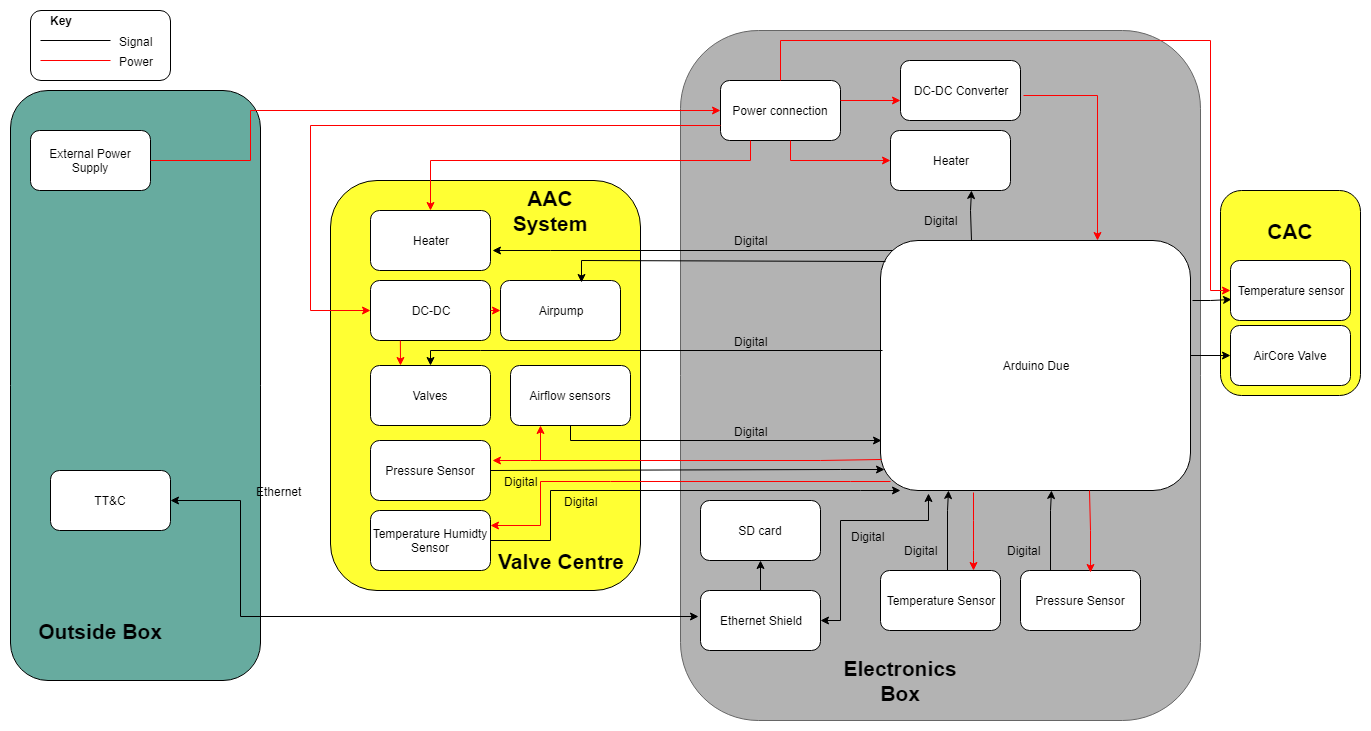
\includegraphics[width=16cm]{4-experiment-design/img/eee-block-diagram-march.png}
    \end{align*}
    \caption{Block Diagram for all Electronic Components Showing the Signal and Power Connections}\label{fig:electronics-block-diagram}
\end{figure}


\begin{figure}[H]
    \begin{align*}
        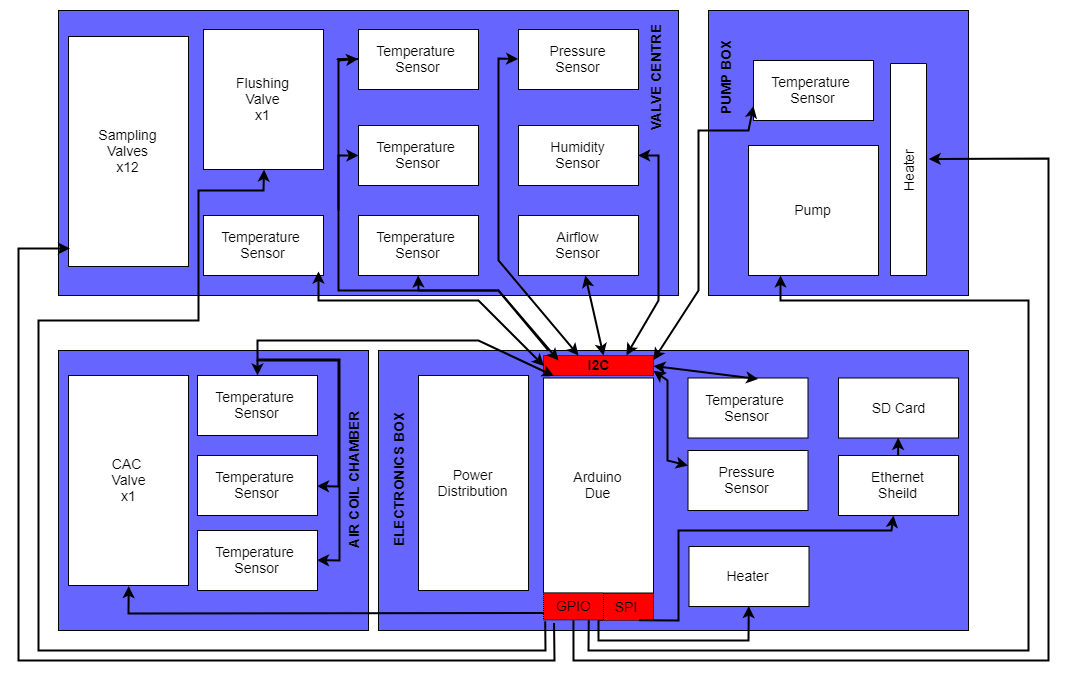
\includegraphics[width=16cm]{4-experiment-design/img/eee-interface-diagram.png}
    \end{align*}
    \caption{Block Diagram Showing the Interfaces Between All Electrical Components.}\label{fig:eee-interface-diagram}
\end{figure}

\begin{centering}
Three DC-DC converters will be used to step down the voltage from the 28.8V provided by the gondola down to: 
\end{centering}

\begin{centering}
\begin{itemize}
  \item $28.8V \Longrightarrow 12V$ for the Arduino.  
  \item $28.8V \Longrightarrow 24V$ for the valves.
  \item $28.8V \Longrightarrow 24V$ for the pump.
  \end{itemize}

\end{centering}
\bigskip

\begin{centering}
The heaters will not require the voltage to be stepped down and so will be powered directly from the gondola battery.
\end{centering}
\bigskip

\subsubsection{Miniature Diaphragm Pump}
PLACE HOLDER. INFORMATION AND PICTURE WILL BE PLACED HERE BEFORE MONDAY.

\subsubsection{Solenoid Valves}
PLACE HOLDER. INFORMATION AND PICTURE WILL BE PLACED HERE BEFORE MONDAY.

\subsubsection{Valve Driving Circuit}
PLACE HOLDER. CIRCUIT DIAGRAM AND EXPLANATION WILL BE PLACED HERE BEFORE MONDAY.

\raggedbottom